\documentclass[12pt,letterpaper]{article}
\usepackage[utf8]{inputenc}
\usepackage{graphicx}
\usepackage{physics}
\usepackage{amsmath}
\usepackage{amssymb}
\usepackage{hyperref}
%\graphicspath{/images/Logpt1.png}
\graphicspath{{./images/}}
\title{CMPT 419 Graphical Models/ Recurrent Neural Networks}
\author{Echo Liu}
\date{Fall 2018}

\let\oldhat\hat
\renewcommand{\vec}[1]{\mathbf{#1}}
\begin{document}
\begin{titlepage}
\maketitle
\end{titlepage}

\section{Question 1: Graphical Models}
\begin{enumerate}
	\item See Appendix section

	\item $P(A,L,G,E,T) = P(T)*P(A|T)*P(E|L,G)*P(L)$

	\item At Node T it is simply a Linear Gaussian $\frac{1}{\sqrt{2*\pi*\sigma^{2}}} * e^\frac{-(x-\mu)^{2}}{2*\sigma^{2}}$
	\\ At Node A it is a sigmoidal distibution with the following form $\frac{1}{1+ exp(g+\sum_{n=1}^{K}w_{n}*z_{n})}$ where the parents are T and E
	\\ At Node E it is a Gaussian as follows, we use $L=0$ to denote non-university and $L=1$ to denote u and the same analogy applies for the current provincial government random variable G, 
	\\ $L(E|L=0,G=0) \sim\ N(A,B)$
	\\ $L(E|L=0,G=1) \sim\ N(C,D)$
	\\ $L(E|L=1,G=0) \sim\ N(E,F)$
	\\ $L(E|L=1,G=1) \sim\ N(G,H)$
	\\ As for the values of the respective parameters, it can be guessed that one would assign a larger
	
	\\ $\mu$ for the Node T as it can be argued that there is more emphasis on the Tuition distribution when deciding whether or not to enroll in SFU. Furthermore, larger weighting 
	\\ will be given to the T parent in the Sigmoidal distribution as despite economy size, tuition becomes a larger deciding factor and the parameters for the Gaussian can be arbritary. 
	\\ Some example values I'd use A=10, B=4, C=8,D=3, E=5, F=9, G=10, H=15.
	%\item At Node T it is simply a Linear Gaussian with $\frac{1}{\sqrt{2*\pi*\sigma^{2}}}$

	\item We need to moralize our graph and realize that the only elements that are relevant are the intermediate parents at each of the nodes.

\end{enumerate}

\section{Question 2: KL Divergence}


\begin{enumerate}

	\item This is essentially the case when the two distributions are equal 
	\\ i.e $p(x)=q(x)$ As such when both distributions are equal the log inside
	\\ the KL formula i.e $\frac{log(p(x))}{log(p(x))}$ 
	
	\item No

	\item We take the proof outlined in this \href{https://stats.stackexchange.com/questions/66271/kullback-leibler-divergence-of-two-normal-distributions?fbclid=IwAR1MGg0ZK6zeZOoYY4Sy6MWnmH1XGirg99kZOdCrfkarrLO8y9FAqG0Dsks}{Stats Stack Exchange} post and change the "+" sign to a minus
	\\ sign and change it to a "-" sign and since our mu terms equal they also zero out plus our 
	\\ 0.5 terms zero out
	\\ $log(\frac{\sigma_{2}}{\sigma_{1}})+\frac{\sigma_{1}^{2}}{2*\sigma_{2}^{2}}-log(\frac{\sigma_{1}}{\sigma_{2}})-\frac{\sigma_{2}^{2}}{2*\sigma_{1}^{2}}$
	\\ $log(\frac{\sigma_{2}^{2}}{\sigma_{1}^{2}})+ \frac{\sigma_{1}^{2}}{2*\sigma_{2}^{2}} -\frac{\sigma_{2}^{2}}{2*\sigma_{1}^{2}}$
	\\ We then use the above equation and make the term inside the log our x

\end{enumerate}

\section{Question 3: Gated Recurrent Unit}

\begin{enumerate}

\item When both are zero. 

\item The hidden state at that time step will be also zero, i.e that GRU forgets everything. 

\end{enumerate}

\section{Appendix}
	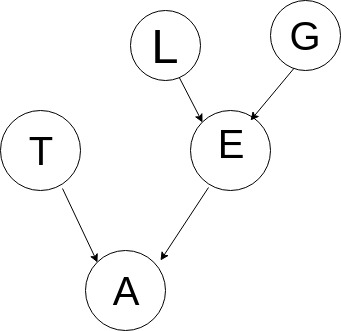
\includegraphics[width=\textwidth]{BayesNetwork}
	\centering
\end{document}
